\section{Speech Waveform Quantization}
\subsection{Evaluation of the optimal k}
In this part we design a Uniform Scalar Quantizer (USQ) that is adapted to the speech signal. For that we define \[xmax = k\sigma_x\] where $\sigma_x^2$ is the variance of the speech signal. This kis to be calculate for everybit rate we choose. The value of k for a bitrate R = 3 is 2.57. The figure \ref{optimalk} shows a plot of SNR = f(k). The SNR has been evaluate with the following formula \[ SNR = \frac{\sigma_x^2 }{\frac{1}{N}\sum_{n=1}^N(x_n - q_R(x_n))^2 } \] where N is the size of the input speech signal, $x_n$ is the input speech signal, $q_R(x_n)$ is the input signal quantized with a bitrate R. Here R=3.


\begin{figure}[h!]
\centering
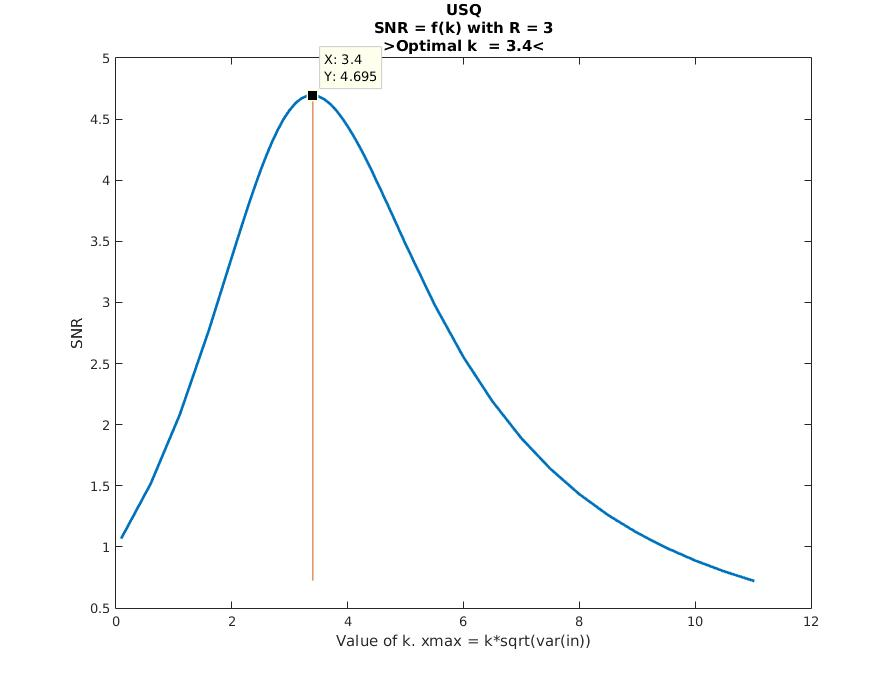
\includegraphics[scale = .4]{optimalk_3bits}
\caption{SNR = f(k) for a bitrate R = 3}
\label{optimalk}
\end{figure}

\subsection{Rate - SNR curve}
The curve ploted on figure \ref{rateSNR}, represents the rate versus the $SNR_{dB}$. The $SNR_{dB}$ has beenevaluated with the following formula : \[ SNR_{dB} = 10log_{10}\frac{\sigma_x^2}{\frac{1}{N}\sum_{n=1}^N(x_n - q_R(x_n))^2}\] where N is the size of the input speech signal, $x_n$ is the input speech signal, $q_R(x_n)$ is the input signal quantized with a bitrate R.

\begin{figure}[h!]
  \centering
  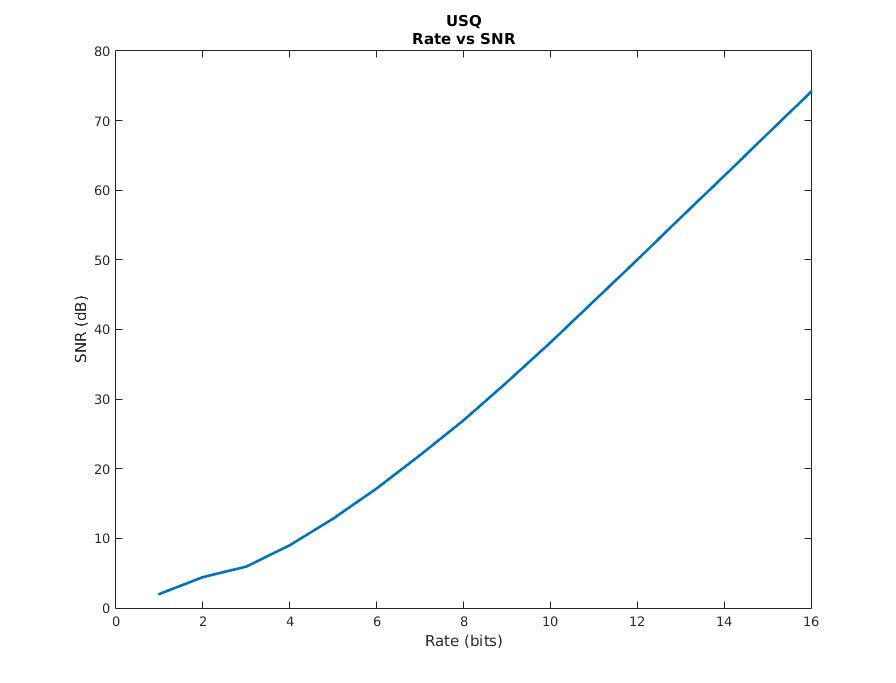
\includegraphics[scale = .4]{rateSNR}
  \caption{Rate versus SNR curve, for rate = \{1,2,$\dots$,16\}}
  \label{optimalk}
\end{figure}

\subsection{Quality of the quantized signal}
A bit rate of 8 bits provides a good quality for the quantized signal.
\subsection{Error signal}
For a bit rate of 1 bit, the error signal contains of the information. It is easier to unserstand the message by listening to the error signal than listening to the quantized signal. The error signal is then highly correlated with the input signal. That compromises one of the fundamental assumptions when we want to remove an additive noise on a signal. On the otherhand when the rate is high, say 11 bits, the error signal sounds like a white noise and is consequently totally decorrelated with the input signal.

\subsection{OPTIONAL:}
With a midtreat quantizer, the message is more understandable a low bitrate and at high bitrate there are no differences. The figure \ref{midtreat} shows the selected levels for a 2 bits midtreat quantizer.
\begin{figure}[h!]
  \centering
  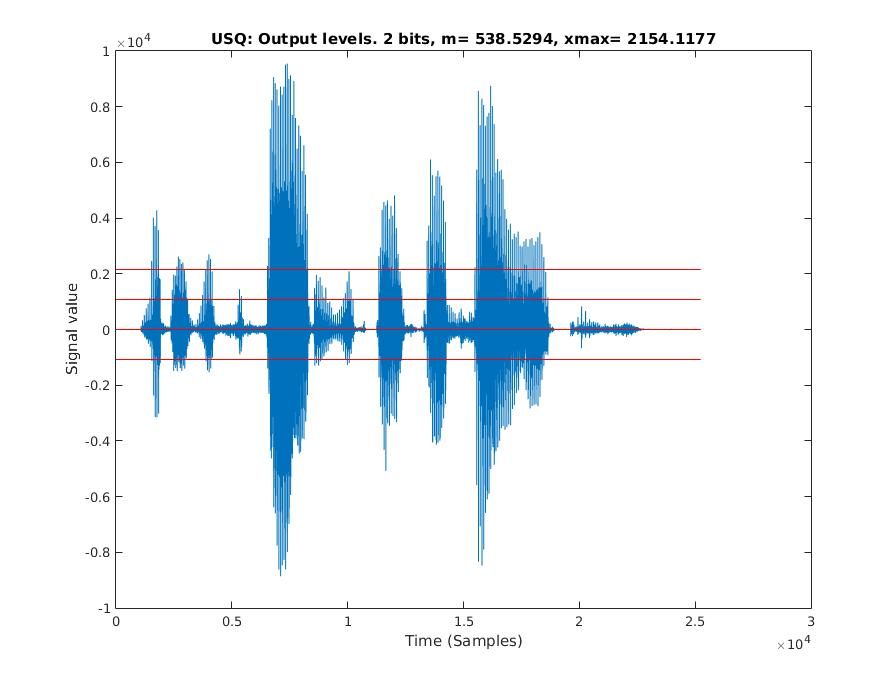
\includegraphics[scale = .4]{midtreat}
  \caption{Midtreat quantizer for R = 2}
  \label{midtreat}
\end{figure}

%%% Local Variables:
%%% TeX-master: "master"
%%% End:
